%
%

%%-----------------------------------------------------
%%-----------------------------------------------------
\section{Unified Modeling Language}

%%-----------------------------------------------------
\begin{frame}
\frametitle{Características}

\begin{itemize}
  \item Lenguaje de modelado de sistemas software
  \item Respaldado por el OMG (Object Management Group)
  \item Gráfico
  \item Sirve para visualizar, especificar, construir y documentar
  \item Pretender ser el ``plano'' que tienen los arquitectos
\end{itemize}

\end{frame}


%%-----------------------------------------------------
\begin{frame}
\frametitle{Diagrama de Clases}

\begin{center}
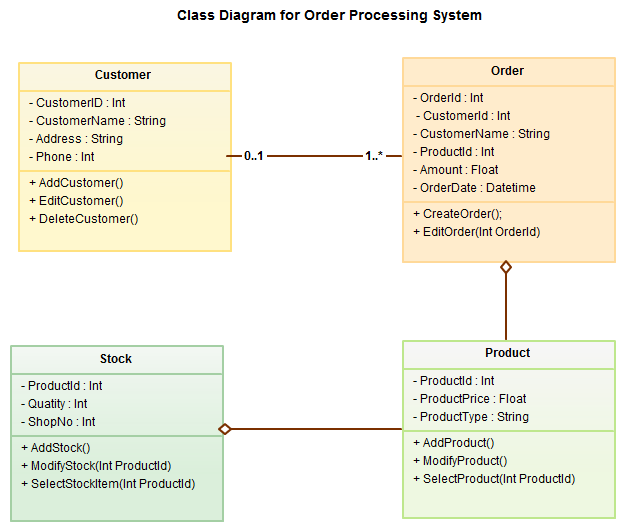
\includegraphics[width=9cm]{figs/UML-Class-Diagram-Example.png}
\end{center}
  
\end{frame}

%%-----------------------------------------------------
\begin{frame}
\frametitle{Diagrama de Paquetes}

\begin{center}
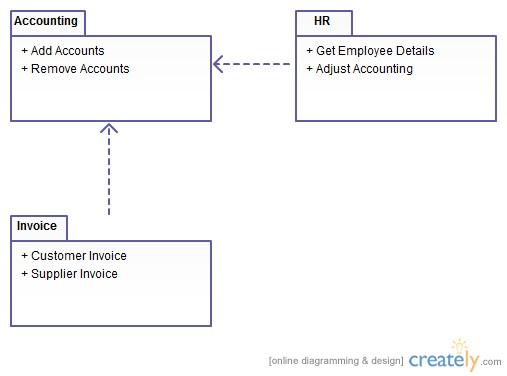
\includegraphics[width=10cm]{figs/Package-Diagram-UML.jpeg}
\end{center}  

\end{frame}

%%-----------------------------------------------------
\begin{frame}
\frametitle{Diagrama de Casos de Uso}

\begin{center}
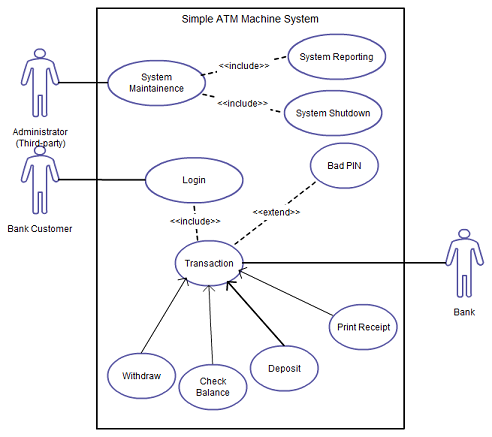
\includegraphics[width=8cm]{figs/Use-Case-Diagram.png}
\end{center}
  
\end{frame}

%%-----------------------------------------------------
\begin{frame}
\frametitle{Diagrama de Secuencia}

\begin{center}
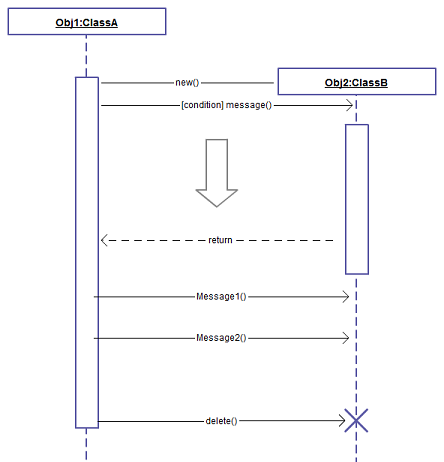
\includegraphics[width=6cm]{figs/Sequence-diagram-UML.png}
\end{center}
  
\end{frame}

%%-----------------------------------------------------
\begin{frame}
\frametitle{Software para UML}

\begin{itemize}
  \item Libre
  \begin{itemize}
    \item ArgoUML
    \item Dia
    \item UML Designer...
  \end{itemize}
  \item Privativo
    \begin{itemize}
    \item Rational Rose
    \item MS Visio...
  \end{itemize}
  \item On-line (privativos)
    \begin{itemize}
    \item creately
    \item Gliffy...
    \end{itemize}
\end{itemize}

\end{frame}

